\section{Collezioni}
Il Java Collections Framework (JCF), parte del \inline{package java.util}, gestisce strutture dati e relativi algoritmi.
\begin{figure}[h]
	\centering
	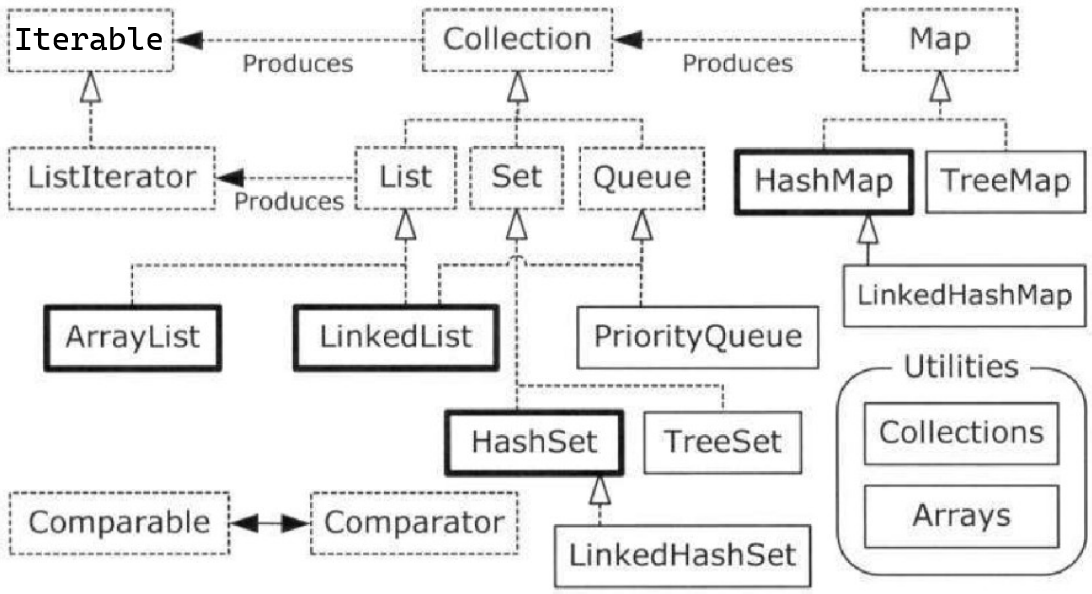
\includegraphics[width=0.8\textwidth]{JCF.png}
\end{figure}

Di nostro interesse sono:
\begin{itemize}
	\item Interfacce: Collection, List, Set, Iterator, Comparable.
	\item Classi: ArrayList, LinkedList, HashSet, HashMap.
	\item Classi Funzionalità: Collections, Arrays.
\end{itemize}

Fondamentalmente ci vengono fornite le collezioni (List, Set, Queue) e Map.

Tutti con un generic.

map: funzioni che metoono in relazione elementi di due gruppi.

in java le collezioni sono tutte mutabili, ovvero si possono modificare gli elementi.

tutte hanno add e toString().

\subsection{Iterable e Iterator}
\colTwo{Una classe che implementa l'interfaccia \textbf{\inline{Iterable<X>}} può essere iterata.}{Una classe di supporto che implementa l'interfaccia \textbf{\inline{Iterator<X>}} dice come essere iterata.}{45}{45}

\multiline{}{}{CodiciEsempio/Iterable.java}

Le due classi usate insieme possono iterare collezioni.

Esempio d'uso è nel foreach, che conosce le due interfacce, è può iterare qualunque oggetto di una classe che implementa \inline{Iterable<X>} e che usa un oggetto di una classe che implementa \inline{Iterator<T>}.

\subsection{Collection}
Interfaccia radice gerarchia interfacce di collezione (gruppi oggetti), estende \inline{Iterable}, e definisce:
\begin{itemize}
	\item Un costruttore vuoto. Assunto implicito.
	\item Un costruttore che accetta una Collection per l'inizializzazione. Assunto implicito.
	\item Operazioni di modifica opzionali.
	\item Operazioni di ricerca basete su Object.equals().
\end{itemize}

\multiline{}{}{CodiciEsempio/Collectoce.java}

I metodi \inline{contains e remove} applica il metodo \inline{Object.equals()} all'oggetto passato con tutti gli elementi della collezione.
Come argomento accetta \inline{Object} per poter confrontare oggetti anche non della stessa classe (potenzialmente uguali per le regole di confronto).

\subsubsection{Collezioni immutabili}
L'unico modo per creare una collezione di valori non modificabili ma solo leggibili.

\oneline{final ... = Set.of| copyOf(...);}
\oneline{final ... = List.of|  copyOf(...);}


\inline{Set | List.of| copyOf()} permette che i valori non siano cambianti e \inline{final} fa si che la variabile non sia riassegnata, rendendo il tutto un blocco unico.

\subsection{List}
Collezione estendibili sequenzializzata con indice. Aggiunge metodi per accesso elementi secondo posizione (O-based). Sono permesse ripetizioni di elementi (anche null).

Estende l'interfaccia \inline{ListIterator<E>} che estende \inline{Iterator<T>} permettendo di scorrere gli elementi sia "in avanti" che "in dietro".

\medskip

Nota: Scandire quando possibile elemnti via iteratore e non indici.

\medskip

Implementazioni sono ArrayList (O(1) tranne add O(n) ammortizzato), con \inline{trimToSize()| ensureCapacity()}, e LinkedList che implementa l'interfaccia Queue (FIFO o LIFO) e Deque.

\subsection{Set}
Collezione estendibili senza ordine e duplicati (\inline{Object.equals()} sempre \inline{false} e al massimo un \inline{null}). Non aggiunge metodi a Collection.

Per migliorare le prestazioni di \inline{contains()} si usa l'approccio \textbf{HashSet (O(1) aromtizzato)} che lega oggetto e posizione, o \textbf{TreeSet (O(logn))}.

Nota: I costruttori di HashSet accettano la dimensione iniziale stimata e un fattore di crescità, se basso hashing veloce, se alto hashing risparmia memoria.

\subsubsection{Ordinamento}
Per rendere gli oggetti di una classe ordinabili possiamo definire il criterio d'ordinamento:
\begin{itemize}
	\item \textbf{Interno} alla classe tramite l'implementazione dell'interfaccia \inline{Comparable<T>}.
	\multiline{}{}{CodiciEsempio/Comparable.java}

	Permette di comparare due oggetti dello stesso tipo secondo un unico criterio.

	\oneline{obj1.compareTo(obj2);}

	\item \textbf{Esterno} alla classe tramite una classe comparatore che implementa l'interfaccia \inline{Comparator<T>}.
	\multiline{}{}{CodiciEsempio/Comparator.java}

	Permette di comparare due oggetti dello stesso tipo secondo tanti criteri quante sono le classi comparatore.

	\oneline{objComparator.compare(obj1, obj2);}
\end{itemize}

Sia \inline{compareTo} che \inline{compare} restituiscono 0 se i due oggetti sono guali, un numero positivo se this o o1 è maggiore oppure un numero negativo se this o o1 è minore.

TreeSet e tante altre classi sfruttano l'ordinamento tra gli oggetti.

\subsection{Moduli}
Le classi statiche Array e Collections forniscono funzioni di base.

Array ha varie versioni di metodi per supportare tutti i tipi mentre Collections ne ha una per tutti.

\subsection{Map}
Collezioen estendibile di funzioni che mappano  Key in Value.

\oneline{public interface Map<K,V> {...}}

Map è biunivoca, due Value diversi non possono avere la stessas Key.

Implementazioni: HashMap, TreeMap.

\subsubsection{Map.Entry}
La mappa, internamente, ha un Set di Entry (coppie chiave-valore). Entry è una StaticNested \inline{interface}.

\multiline{}{}{CodiciEsempio/map.java}

Quindi per iterare una mappa si usa $entrySet()$ e il tipo degli elementi è $Map.Entryz<K, V>$.